\documentclass{article}
\usepackage[margin=1in, bottom=0.5cm, top=1cm, paperwidth=8.5in, paperheight=11in]{geometry}
\usepackage{multicol}
\usepackage{amsmath}
\usepackage{graphicx}
\usepackage{float}

\title{Transformers Mate Just Fine}
\author{Patrik Friedlos\\FHNW CAS Deep Learning Vertiefungsprojekt}
\date{January 2025}

\begin{document}
\maketitle

\begin{abstract}
We partially reproduce recent research on using transformers to learn state values in chess. A "mateness" target is explored that alleviates the reported shortcoming of indecisiveness in the face of overwhelming victory. We demonstrate improved playing strength of the resulting policy.
\end{abstract}

\begin{multicols}{2}

\section{Introduction}

In recent years, Deep Learning has become ubiquitous in computer chess. The world's strongest chess engine Stockfish uses neural networks for position evaluations since 2020. Alpha Zero and Leela Chess Zero use deep reinforcement learning combined with Monte Carlo tree search. Recently, Google Deep Mind trained transformer models for chess. The resulting policies yield grandmaster-level chess without reliance on a search algorithm \cite{ruossamortized}.

\section{Method}

We partially reproduce the state-value approach by Ruoss et al. by training a transformer model on ChessBench. The implementation follows the paper, but we use a 64x64 board representation instead of FEN strings. Additionally, we annotate the dataset with a "mateness" score by evaluating all positions that are close to mate with Stockfish up to 10 ply. Mateness is then defined as:

$m = \left\{
\begin{array}{ll}
1 - n_m / d & \textrm{if mate found} \\
0 & \, \textrm{else} \\
\end{array}
\right. $

Where $n_m$ is the number of moves until mate and $d$ is the depth searched. Mateness is trained with a binary cross entropy loss and the policy is constructed by using the sum of the expected win probability and the mateness.


\section{Results}

We evaluate the playing strength of the engine in 1000 games against Stockfish 17 at 2000 ELO (CCRL Blitz) and report an ELO of 2191 (without mateness) and 2323 (with mateness) using Ordo. We get an accuracy of 79.5\% (without mateness) and 79.9\% (with mateness) on the Lichess puzzle dataset.

\section{Discussion}

We have seen that shortcomings of the no-search transformer approach to chess in terms of indecisiveness in the face of overwhelming victory can be reduced by introducing an additional mateness target. This increases the playing strength of resulting policies, arguably because the engine more easily converts winning positions, as an example in Figure 1 shows. The small improvement on the puzzle dataset is probably due to the fact that there is only one (objectively obvious) solution to puzzles, and hence mateness can't tip the scale among many winning moves. We only annotated the dataset to a maximum of 10 plies and trained a small transformer model (3.7M parameters). Hence there is an opportunity to further refine the approach.

\begin{figure}[H]
  	\centering
    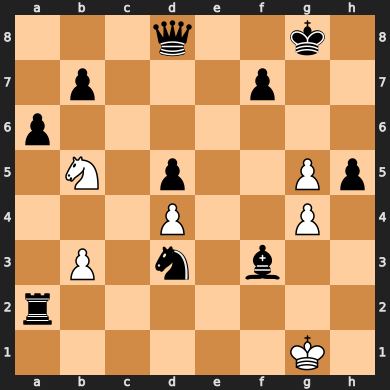
\includegraphics[width=0.25\textwidth]{example.png}
    \caption{A position the engine drew as black. Using mateness it plays Qxd4 and wins in 3 moves.}
\end{figure}

\section{Conclusion}

Using mateness as an additional target for a transformer playing chess without search can improve playing strength by reducing indecisiveness in the face of overwhelming victory.

\bibliography{refs} 
\bibliographystyle{ieeetr}

\end{multicols}

\end{document}